\subsection{Comparación entre todos los ejemplos}

	Para una mejor comprensión de la eficacia del RNA y el ACG como herramienta para el análisis y generación de señalamiento, los resultados obtenidos en el ejemplo 1 son contrapuestos junto a los resultados de los ejemplos 2 al 9. Estos ejemplos extra pueden encontrarse detallados en los Apéndices comprendidos entre el Apéndice \ref{sec:ejemplo_2} (ejemplo 2) y el Apéndice \ref{sec:ejemplo_9} (ejemplo 9). La comparación entre los ejemplos generados se puede visualizar en la Tabla \ref{Tab:tabla_ACG_total}.

	\begin{table}[H]
		{
			\caption{Comparación entre los ejemplos generados por el ACG.}
			\label{Tab:tabla_ACG_total}
			\centering
			%\small
			%\centering
			\begin{center}
				\resizebox{1\textwidth}{!}{
					\begin{tabular}{ c c c c c c c c c c  }
						\hline	
						Recursos & Ejemplo 1 & Ejemplo 2 & Ejemplo 3 & Ejemplo 4 & Ejemplo 5 & Ejemplo 6 & Ejemplo 7 & Ejemplo 8 & Ejemplo 9\\	
						\hline
						netElements 	& 11  & 7  & 53  & 47  & 8  & 11 & 7 & 5 & 7\\
						borders 		& 4   & 4  & 18  & 5   & 0  & 2  & 0 & 4 & 0\\
						bufferStops		& 3   & 1  & 12  & 14  & 4  & 5  & 5 & 0 & 2\\
						levelCrossings 	& 2   & 1  & 1   & 2   & 0  & 0  & 0 & 6 & 3\\
						platforms 		& 2   & 2  & 13  & 0   & 0  & 0  & 0 & 2 & 5\\
						singleSwitch 	& 5   & 3  & 15  & 22  & 4  & 5  & 3 & 2 & 4\\
						doubleSwitch 	& 0   & 0  & 2   & 1   & 0  & 0  & 0 & 0 & 0\\
						scissorSwitch 	& 0   & 0  & 1   & 0   & 0  & 0  & 0 & 0 & 0\\
						\hline
						signals 		& 23  & 12 & 82  & 77  & 16 & 24 & 13 & 16 & 25\\
						routes 		 	& 21  & 10 & 91  & 89  & 16 & 22 & 11 & 13 & 27\\
						\hline
						N 				& 62  & 33 & 245 & 238 & 44 & 62 & 34 & 42 & 66\\
						\hline
						LUT 			& 3416  & 1793  & 13509 & 13666 & 2307  & 3348  & 1798  & 2164  & 3829\\
						FF 				& 3813  & 1993  & 15113 & 15072 & 2347  & 3796  & 2011  & 2284  & 4137\\
						IO 				& 15    & 15    & 15    & 15    & 15    & 15    & 15    & 15    & 15\\
						BUFG 			& 3     & 3     & 3     & 3     & 3     & 3     & 3     & 3     & 3\\
						\hline
						\% LUT 			& 6,42  & 3,37  & 25,39 & 25,69 & 4,34  & 6,29  & 3,38  & 4,07  & 7,20\\
						\% FF 			& 3,58  & 1,87  & 14,20 & 14,17 & 2,21  & 3,57  & 1,89  & 2,15  & 3,89\\
						\% IO 			& 12,00 & 12,00 & 12,00 & 12,00 & 12,00 & 12,00 & 12,00 & 12,00 & 12,00\\
						\% BUFG 		& 9,38  & 9,38  & 9,38  & 9,38  & 9,38  & 9,38  & 9,38  & 9,38  & 9,38\\
					\end{tabular}
				}
			\end{center}
		}    
	\end{table}
	
	Debido a que se utiliza una interfaz serie para comunicar los datos, la cantidad de pines utilizados es independiente del tamaño del sistema a a implementar, lo cual se refleja en el número de pines de entrada y salida (IOs) y de buffers (BUFGs). Sin embargo, la cantidad de Look-Up-Tables (LUTs) y Flip-Flops (FFs) incrementa considerablemente. En la Figura \ref{fig:ACG_RECURSOS_1} se puede visualizar la cantidad de Look-Up-Table y Flip-Flops utilizadas en función de la cantidad de elementos ferroviarios (N). La cantidad de recursos utilizados incrementa linealmente, a diferencia del enfoque funcional explicado en la Sección \ref{sec:funcional}, cuyo crecimiento es exponencial.	
	 	
	\begin{figure}[H]
		\centering
		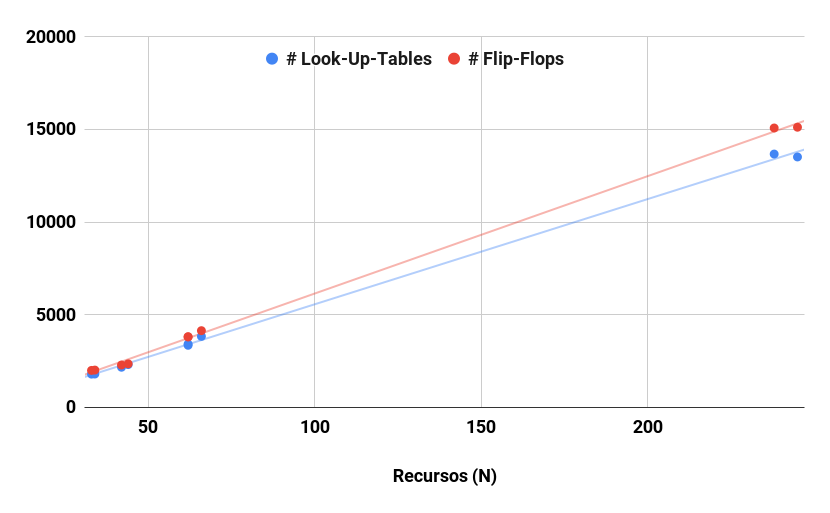
\includegraphics[origin = c, width=0.9\textwidth]{resultados-obtenidos/ejemplo1/images/recursos_1}
		\centering\caption{Uso de Look-Up-Tables (LUTs) y Flip-Flops (FFs) en función de N.}
		\label{fig:ACG_RECURSOS_1}
	\end{figure}
	
	En la Figura \ref{fig:ACG_RECURSOS_2} se visualizan los mismos datos de la Figura \ref{fig:ACG_RECURSOS_1}, esta vez ponderados por la cantidad de recursos disponibles en la plataforma Arty Z7 20.
	
	\begin{figure}[H]
		\centering
		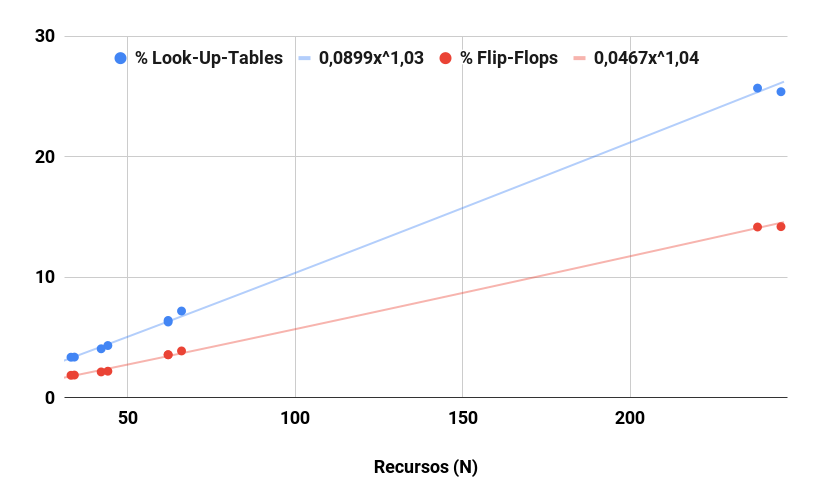
\includegraphics[origin = c, width=0.9\textwidth]{resultados-obtenidos/ejemplo1/images/recursos_2}
		\centering\caption{Porcentaje de uso de Look-Up-Tables (LUTs) y Flip-Flops (FFs) en función de N, considerando la plataforma Arty Z7 20.}
		\label{fig:ACG_RECURSOS_2}
	\end{figure}
	
	Realizando una aproximación lineal podemos calcular el valor de N para el cual el uso de la plataforma alcanza el 100\%. Si consideramos la cantidad de Flip-Flops, un valor de N igual a 1684 sería suficiente para que el proceso de implementación fallase por falta de recursos disponibles. Si consideramos la cantidad de Look-Up-Tables, el valor límite de N es 937. Por lo tanto, siendo que el ejemplo mas grande implementado es, según la Tabla \ref{Tab:tabla_ACG_total}, el ejemplo 3 con un valor de N de 245, se podría implementar un sistema hasta 3,8 veces mas grande sin inconvenientes.
	
	 Si consideramos un sistema 3,8 veces mas grande que el ejemplo 3 estaríamos hablando de una red ferroviaria de 49 estaciones, 68 cambios de vías, 193 secciones de vías, 311 semáforos y hasta 345 rutas. A modo de referencia, la línea Roca, la mas extensa del área metropolitana de Buenos Aires, cuenta con 69 estaciones a lo largo de mas de 230 kilómetros \cite{TRENES}. Por lo que un hipotético ejemplo que utilice el 100\% de la plataforma cubriría el 71\% de todas las funcionalidades de dicha linea.
	